\section{Theorie}

\section{Durchführung}
\section{Auswertung}


%gucken Punkte Komma
\subsection{Eichung des Elektromagneten}
Um die Magentfeldstärke im Inneren des Elektromagneten zu bestimmen, wird eine nichtlineare Regression der Form

\begin{equation}
  B(I) = a_0 + a_1 \cdot I + a_2 \cdot I² + a_3 \cdot I³
  \label{eq:B}
\end{equation}
durchgeführt. Diese liefert die Werte der Koeffizienten:

\begin{align*}
  a_0 &= \SI{5(5)}{\milli\tesla} \\
  a_1 &= \SI{59.0(18)}{\milli\tesla\per\ampere} \\
  a_2 &= \SI{0.80(19)}{\milli\tesla\per\ampere²} \\
  a_3 &= \SI{-0,053(6)}{\milli\tesla\per\ampere³}
\end{align*}
Die Messwerte und der Fit sind in Abbildung \ref{abb:1} und Tabelle \ref{tab:1} zu sehen.

\begin{table}
  \centering
  \caption{Messwerte zur Eichung des Elektromagneten.}
  \label{tab:1}
  \begin{tabular}{c c | c c}
    \toprule
    $I$ / \si{\ampere} & $B$ / \si{\milli\tesla} & $I$ / \si{\ampere} & $B$ / \si{\milli\tesla} \\
    \midrule
    0 & 4  & 12 & 742 \\
    1 & 62 & 13 & 806 \\
    2 & 124 & 14 & 839 \\
    3 & 197 & 15 & 891 \\
    4 & 250 & 16 & 935 \\
    5 & 307 & 17 & 980 \\
    6 & 379 & 18 & 1018 \\
    7 & 434 & 19 & 1050 \\
    8 & 509 & 20 & 1079 \\
    9 & 552 & 21 & 1108 \\
    10 & 611& 22 & 1132 \\
    11 & 680 \\
    \bottomrule
  \end{tabular}
\end{table}

\begin{figure}
  \centering
  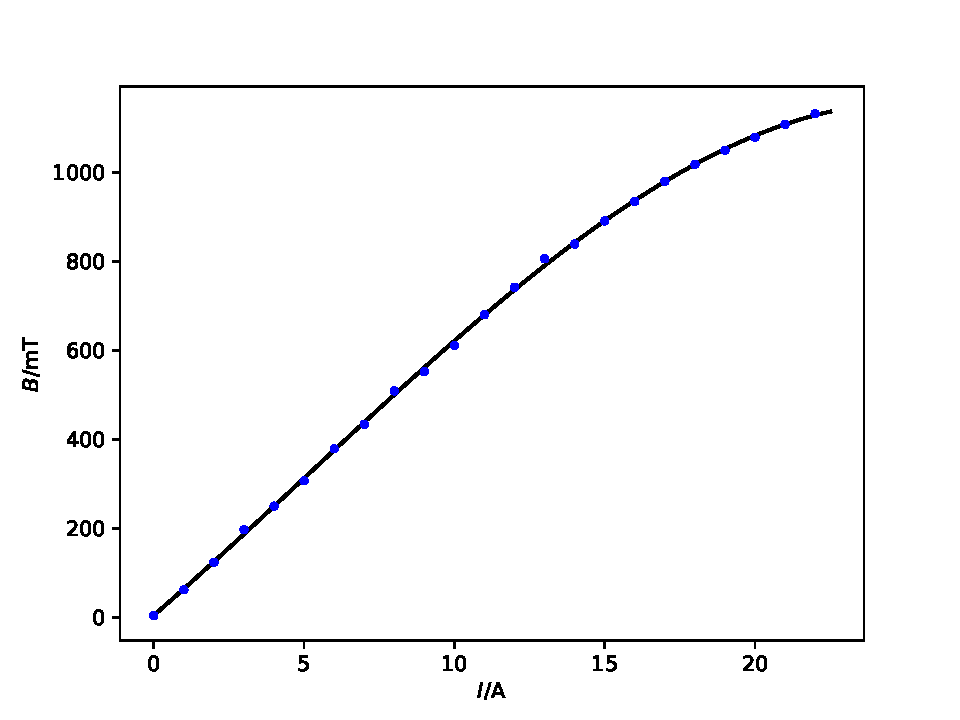
\includegraphics[scale=0.7]{Magnetfeld.pdf}
  \caption{Fit und Messwerte zur Eichung des Elektromagneten.}
  \label{abb:1}
\end{figure}


\subsection{\texorpdfstring{Zur Berechnung der $\symup{\Delta}(m \cdot g)$}{}-Werte}
Die bekannte Formel
\begin{equation*}
  E(\lambda) = \frac{hc}{\lambda}
\end{equation*}
zur Berechnung der Energie einer elektromagnetischen Welle aus deren Wellenlänge $\lambda$
sowie dem $\textsc{Planck}$schen Wirkungsquantum $h$ und der Vakuumlichtgeschwindigkeit $c$
ist offensichtlich nicht linear in $\lambda$. Da für diese Auswertung jedoch ein Wert
$\symup{\Delta} E(\symup{\Delta} \lambda)$ notwendig ist um nach:
\begin{equation}
  \symup{\Delta} E = \underbrace{ \{m_1 g_1 - m_2 g_2 \} }_{\substack{\symup{\Delta}(m \cdot g)}}
  \mu_B B
  \label{eq:2}
\end{equation}
aus einer Magnetfeldstärke $B$ und dem $\textsc{Bohr}$schen Magenton einen Wert $\symup{\Delta}(m \cdot g)$
zu berechnen, muss die Ableitung $\frac{\partial}{\partial \lambda} E$ bestimmt werden da
ein Gleichsetzen der beiden Ausdrücke für $E$ aufgrund der erwähnten nicht-Linearität verboten ist.
Aus der Ableitung folgt:
\begin{equation}
  \frac{\partial}{\partial \lambda} E = -\frac{h c}{\lambda^2} \Leftrightarrow
  \symup{\Delta} E = -\frac{h c}{\lambda^2} \symup{\Delta} \lambda.
  \label{eq:3}
\end{equation}
Dieser Ausdruck ist nun abhängig von der konstanten unverschobenen Wellenlänge
$\lambda$ und linear in der Wellenlängenverschiebung $\symup{\Delta} \lambda$. Ein Gleichsetzen der
Ausdrücke \eqref{A_eq:2} und \eqref{A_eq:3} ist daher erlaubt und liefert:
\begin{equation}
  |\symup{\Delta}(m \cdot g)| = \frac{h c}{\lambda^2 \mu_B B} \symup{\Delta} \lambda.
  \label{eq:4}
\end{equation}


\subsection{Auswertung der roten Linie}

Zur Auswertung werden die Abstände $\symup{\Delta} s$ der Linien ohne Magnetfeld und die Abstände $\symup{\delta} s$ der aufgespaltenen Linien mit Magnetfeld ausgemessen.
Da der Abstand zwischen zwei Linien vermessen wird, aber sich je eine Linie durch das Magnetfeld in zwei aufspaltet, muss der Mittelwert der jeweils
angrenzenden $\symup{\delta} s$ genommen werden. Die Abstände sind in Tabelle \ref{tab:2} aufgelistet, wobei die Einheit der Abstände Pixel beschreibt.
%im nächsten Absatz muss noch vernünftig referiert werden
Das Dispersionsgebiet wird mit der Formel \eqref{} berechnet, wobei hier die Wellenlänge $\lambda= \SI{643,8}{\nano\meter}$, die Dicke der
Lummer-Gehrcke-Platte $L=\SI{4}{\milli\meter}$ und der dazugehörige Brechungsindex $n(\SI{643,8}{\nano\meter})= 1,4567$ eingesetzt wird:

\begin{equation*}
  \symup{\Delta}\lambda_{\symup{D, rot}} = \SI{48,91}{\pico\meter}
\end{equation*}

Die Wellenlängenänderung $\symup{\delta}\lambda$ kann somit durch die Formel

\begin{equation}
\symup{\delta}\lambda = \frac{1}{2} \frac{\symup{\delta}s}{\symup{\Delta}s} \cdot \symup{\Delta}\lambda_{\symup{D}}
\label{eq:5}
\end{equation}

berechnet werden. Die berechneten Wellenlängenverschiebungen $\symup{\delta}\lambda$
sind ebenfalls in Tabelle \ref{tab:2} zu finden.
Der Mittelwert der Wellenlängenverschiebung beträgt
$\overline{\symup{\delta}\lambda_{·\symup{rot}}} = \SI{10.89(15)}{\pico\meter}$.

Zu Berechnung des dazugehörigen Landé-Faktors muss die Magnetische Feldstärke B
mit Hilfe der Ausgleichsrechnung zur Eichung des Magnetfeld berechnet
werden (siehe Gleichung \eqref{eq:B})
\begin{equation*}
  B(\SI{9}{\ampere})= \SI{561,64}{\milli\tesla}
\end{equation*}

Der Landé-Faktor kann nun mit Hilfe der Formel \eqref{eq:4} bestimmt werden:

\begin{equation}
  |\symup{\Delta}(m \cdot g)| = \frac{h c}{\lambda^2 \mu_B B} \symup{\Delta} \lambda.
\end{equation}

Mit dem $\textsc{Planck}$schen Wirkungsquantum $h$, der Vakuumlichtgeschwindikeit
$c$, der Wellenlänge $ \lambda = \SI{643,8}{\nano\meter}$, dem Bohrschen
Magneton $\mu_B$ und der Wellenlängeverschiebung $\symup{\Delta}\lambda$ folgt

\begin{equation*}
  |\symup{\Delta}(m \cdot g)_{\symup{rot, \sigma}}| = \SI{1,002(5)}{}.
\end{equation*}

Da es bei dem normales Zeeman-Effekt keine Verschiebung der Linie bei dem
$\pi$-Übergang, wird hier $|\symup{\Delta}(m \cdot g)_{\symup{rot, \pi}}| = 0$
angenommen.

\begin{table}
  \centering
  \caption{Messwerte: Abstände der roten Linie.}
  \label{tab:2}
  \begin{tabular}{c c c}
    \toprule
    $\symup{\Delta}s$ / pix & $\symup{\delta}s$ / pix & $\symup{\delta}\lambda$ / \si{\pico\meter} \\
    \midrule
    392.00 & 170.50 & 10.64 \\
    333.00 & 148.50 & 10.91 \\
    301.00 & 132.50 & 10.77 \\
    267.00 & 118.50 & 10.85 \\
    247.00 & 112.00 & 11.09 \\
    230.00 & 104.00 & 11.06 \\
    220.00 & 97.00 & 10.78 \\
    209.00 & 94.50 & 11.06 \\
    196.00 & 88.50 & 11.04 \\
    193.00 & 83.50 & 10.58 \\
    177.00 & 78.00 & 10.78 \\
    158.00 & 72.00 & 11.14 \\
    \bottomrule
  \end{tabular}
\end{table}

\subsection{Auswertung der blauen Linie}

Zur Auswertung des anormalen Zeeman-Effekts bei der blauen Linie, werden erneut
die Abstände $\symup{\Delta}s$ der Linien ohne Magnetfeld gemessen und
anschließend die Abstände $\symup{\delta}s$ zwischen den durch das Magnetfeld
aufgespalteten Linien. Auch hier muss der Mittelwert der angrenzenden
$\symup{\delta}s$ genommen werden.
Zur Berechnung der Wellenlängenverschiebung muss zunächst das
Dispersiongebiet berechnet werden. Mit Hilfe der Gleichung \eqref{}
%hier noch die Referenz einfügen
\begin{equation*}
  \symup{\Delta}\lambda_{\symup{D, blau}} = \SI{26.95}{\pico\meter}
\end{equation*}

Die Messwerte und die mit Gleichung \eqref{eq:5} berechneten
Wellenlängeverschiebungen sind in Tabelle \ref{tab:2} aufgelistet.
Der Mittelwert der Wellenlängenverschiebung beträgt

\begin{align}
  \overline{\symup{\delta}\lambda_{\symup{blau, \pi}}} = \SI{6.25(17)}{\pico\meter} \\
  \overline{\symup{\delta}\lambda_{\symup{blau, \sigma}}} = \SI{6.31(19)}{\pico\meter} \\
\end{align}

Mit Hilfe der zuvor berechneten Regression für das Magnetfeld im Inneren des
Elektromagneten (siehe Gleichung \eqref{eq:B}) wird die Magentfeldstärke bestimmt:
\begin{align*}
  B(I_{\symup{blau, \pi}}=\SI{21}{\ampere}) = \SI{1108.15}{\milli\tesla} \\
  B(I_{\symup{blau, \sigma}}=\SI{5.5}{\ampere}) = \SI{344.31}{\milli\tesla} \\
\end{align*}



\begin{table}
  \centering
  \caption{Messwerte zur blauen Linie.}
  \label{tab:3}
  \begin{tabular}{c c c|c c c}
    \toprule
    \multicolumn{3}{c}{$\pi$-Übergang} & \multicolumn{3}{c}{$\sigma$-Übergang} \\
    $\symup{\Delta}s_{\pi}$ / pix & $\symup{\delta}s_{\pi}$ / pix & $\symup{\delta}\lambda_{\pi}$ / \si{\pico\meter} &
    $\symup{\Delta}s_{\sigma}$ / pix & $\symup{\delta}s_{\sigma}$ / pix & $\symup{\delta}\lambda_{\sigma}$ / \si{\pico\meter} \\
    \midrule
    380.00 & 155.00 & 5.50 & 306.00 & 168.00 & 7.40 \\
    308.00 & 140.00 & 6.12 & 280.00 & 132.00 & 6.35 \\
    208.00 & 124.00 & 8.03 & 242.00 & 115.00 & 6.40 \\
    238.00 & 106.00 & 6.00 & 228.00 & 101.00 & 5.97 \\
    222.00 & 96.00 & 5.83 & 210.00 & 97.00 & 6.22 \\
    216.00 & 94.00 & 5.86 & 204.00 & 96.00 & 6.34 \\
    188.00 & 92.00 & 6.59 & 246.00 & 89.00 & 4.88 \\
    184.00 & 91.00 & 6.66 & 184.00 & 80.00 & 5.86 \\
    178.00 & 86.00 & 6.51 & 162.00 & 76.00 & 6.32 \\
    168.00 & 80.00 & 6.42 & 166.00 & 74.00 & 6.01 \\
    158.00 & 73.00 & 6.23 & 144.00 & 70.00 & 6.55 \\
    148.00 & 66.00 & 6.01 & 135.00 & 67.00 & 6.69 \\
    \bottomrule
  \end{tabular}

\end{table}
